\writeSectionFrame{\presentationTitle}{Das Problem}

\frameWithImageOnly{\BILDERPFAD/problem1.jpg}
\note{
	Unser Kunde ist die Kette Cafe King. Cafe King bietet eine ganze Menge an Kaffeespezialitäten und Zutaten an. Wir sollen eine Software entwickeln, die leicht erweiterbar ist um weitere Kaffeesorten und Zutaten, denn Cafe King möchte gerne expandieren. 
}


\begin{frame}
    \begin{tikzpicture}
\draw[
    draw=Blue,
    line width=10mm,
    -{Triangle[length=12mm,width=14mm]}
]
(0,0) -- (6cm,0);
\end{tikzpicture}
\end{frame}


\begin{frame}{Klassendiagramm -- 1. Entwurf}
\begin{tikzpicture}[scale=0.6, transform shape]
    \umlclass[x=6, y=0]{Beverage}{
        - description: String \\
    }{
        + getDescription(): String \\
        + calculateCosts():double \\
    }

    % Definiere eine weitere Klasse
    \umlclass[x=0, y=-5]{Espresso}{
    }{
        + calculateCosts():double \\
    }

    \umlclass[x=5, y=-5]{Cappuccino}{
    }{
        + calculateCosts():double \\
    }

    \umlclass[x=10, y=-5]{Coffee}{
    }{
        + calculateCosts():double \\
    }

    \umlclass[x=15, y=-5]{Tea}{
    }{
        + calculateCosts():double \\
    }
    \umlinherit{Cappuccino}{Beverage}
    \umlinherit{Espresso}{Beverage}
    \umlinherit{Coffee}{Beverage}
    \umlinherit{Tea}{Beverage}
\end{tikzpicture}
\end{frame}
\note{
 	Es gibt eine ganze Menge an Kaffeesorten. Von jeder Kaffeesorte wird eine Beschreibung gespeichert und der Preis muss berechnet werden können.
}

\begin{frame}{Klassendiagramm mit Zutaten -- 1. Entwurf}
\begin{tikzpicture}[scale=0.6, transform shape]
    % Definiere eine Klasse
    \umlclass[x=6, y=0]{Beverage}{
        - description: String \\
    }{
        + getDescription(): String \\
        + calculateCosts():double \\
    }

    \umlclass[x=0, y=-2]{PlainTea}{
    }{
        + calculateCosts():double \\
    }

    % Definiere eine weitere Klasse
    \umlclass[x=0, y=-5]{TeaWithSugar}{
    }{
        + calculateCosts():double \\
    }

    \umlclass[x=5, y=-5]{TeaWithMilk}{
    }{
        + calculateCosts():double \\
    }

    \umlclass[x=10, y=-5]{TeaWithMilkAndSugar}{
    }{
        + calculateCosts():double \\
    }

    \umlclass[x=15, y=-5]{CoffeeWithSugar}{
    }{
        + calculateCosts():double \\
    }

    \umlclass[x=12, y=-2]{CoffeeWithMilk}{
    }{
        + calculateCosts():double \\
    }

    \umlclass[x=12, y=0]{CoffeeWithMilkAndSugar}{
    }{
        + calculateCosts():double \\
    }
    \umlinherit{TeaWithSugar}{Beverage}
    \umlinherit{PlainTea}{Beverage}
    \umlinherit{TeaWithMilk}{Beverage}
    \umlinherit{TeaWithMilkAndSugar}{Beverage}
    \umlinherit{CoffeeWithSugar}{Beverage}
    \umlinherit{CoffeeWithMilk}{Beverage}
    \umlinherit{CoffeeWithMilkAndSugar}{Beverage}
\end{tikzpicture}
\end{frame}
\note{
 	So ergeben sich eine unglaubliche Menge an Kombinationsklassen und eine Struktur, die nicht wartbar und erst recht nicht erweiterbar ist. 
}

\begin{frame}{Lösungsvorschlag}
\begin{tikzpicture}[scale=0.6, transform shape]
    % Definiere eine Klasse
    \umlclass[x=6, y=0]{Beverage}{
        - description: String \\
        - milk: boolean \\
        - sugar: boolean \\
        - soy: boolean \\
        - caramel: boolean \\
    }{
        + getDescription(): String \\
        + calculateCosts():double \\
        + hasMilk: boolean \\
        + hasSugar: boolean \\
        + hasSoy: boolean \\
        + hasCaramel: boolean\\
    }

    % Definiere eine weitere Klasse
    \umlclass[x=0, y=-5]{Tea}{
    }{
        + calculateCosts():double \\
    }

    \umlclass[x=5, y=-5]{Cappuccino}{
    }{
        + calculateCosts():double \\
    }

    \umlclass[x=10, y=-5]{Coffee}{
    }{
        + calculateCosts():double \\
    }
    
    \umlinherit{Cappuccino}{Beverage}
    \umlinherit{Coffee}{Beverage}
    \umlinherit{Tea}{Beverage}
\end{tikzpicture}
\end{frame}

\note{
	Folgender Vorschlag wurde unterbreitet: Wir erweitern die Klasse um boolsche Attributen für jede Zutat und die Methode calculateCosts() berechnet aus der Belegung dieser Attribute die Kosten. Die Unterklasse verwenden dann in ihrer Implementierung von calculateCosts() die Methode der Oberklasse. 
}

\begin{frame}{Probleme}
	\begin{itemize}
 		\item Wartungsalptraum
 		\pause
 		\item Unübersichtliche calculateCosts()-Methode
 		\pause
 		\item Schwer zu erweitern
 		\item Verstößt gegen Open-Closed-Prinzip
        \item Änderungen betreffen viele Klassen
 	\end{itemize}
    \vspace{0.3cm}
    \hspace{0.3cm}
    \arrowFazit{1.3}{
        Wir machen jetzt was anders\\
Hier steht das Fazit\\
Cappuccino
    }

\end{frame}

\begin{frame}{Beispiel wowo so ein langer Titel twefwf fscs s dfadf  fsegs s fes}
    \arrowImages{1.5}
    {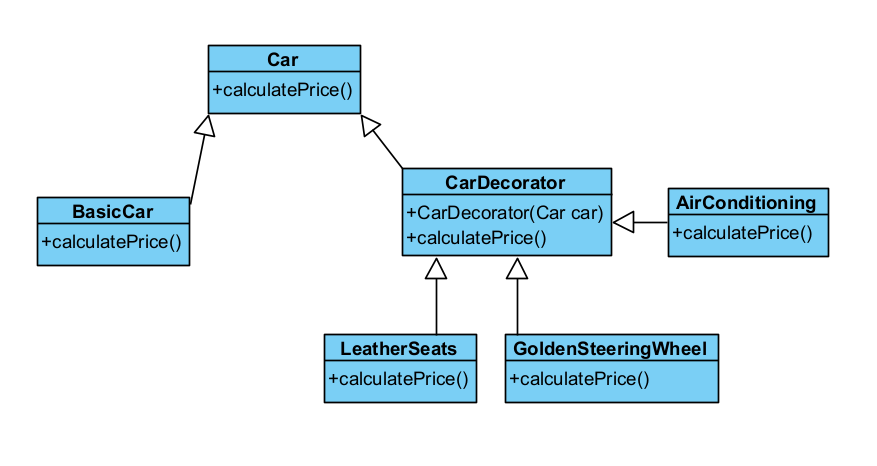
\includegraphics[height=3cm]{5-Decorator/bilder/cpp1.png}}
    {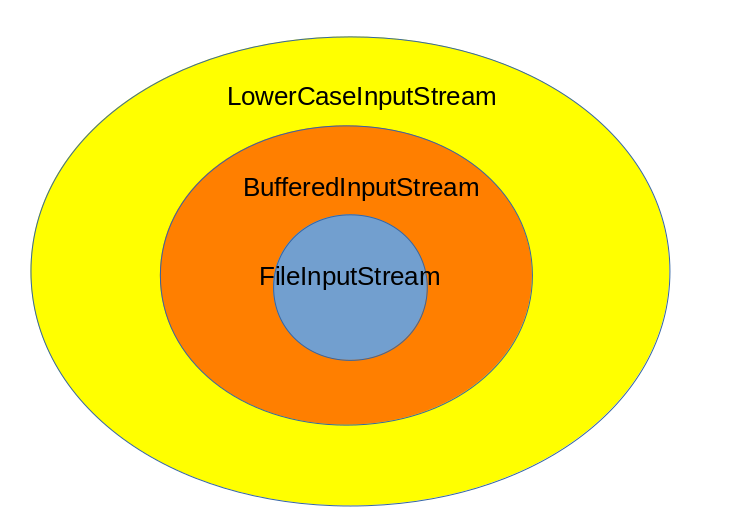
\includegraphics[height=2.8cm]{5-Decorator/bilder/realwelt1.png}}
\end{frame}